%!TEX root = ../thesis.tex
% chapter 1

\chapter{Introduction}
\label{sec:ch1}

Plasma is a macroscopically quasi-neutral fluid composed of partly or fully charged particles \cite{langmuir1928oscillations, bellan2008fundamentals}. Being neutral on both a temporal and spatial scale is one of the important properties of plasma. Unlike fluids such as electron gas, which can be approximated as an ideal gas, attraction and repulsion by electromagnetic force among particles play a crucial role in mechanics. Plasma physics is the field that studies the dynamics of these fluids. There are various research topics, such as finding the equation of the state of plasma or devising ways to deal with collisions between particles.

Plasma physics covers a wide range of research fields and has many practical applications. Since the advent of plasma physics in the early 1900s, it has contributed significantly to increasing the range and productivity of human beings. The spread of plasma light bulbs has extended the available time for human's \cite{de1986high}, the development of low pressure plasma technology is introduced as an essential technology for nano-fabrication of semiconductors \cite{donnelly2013plasma}, and recent research on high temperature plasma leads us to the goal of achieving freedom from energy production through controllable fusion power \cite{mukhovatov1971plasma, fisch1978confining, kwon2011overview}. Meanwhile, plasma physics has always appeared on the journey to satisfy human intellectual curiosity. Various studies are being conducted on an astronomical scale, including understanding the life of stars and planets, finding out the temperature of objects that cannot be reached directly, and predicting the composition of interstellar materials.

\begin{figure}[ht!]
\centering
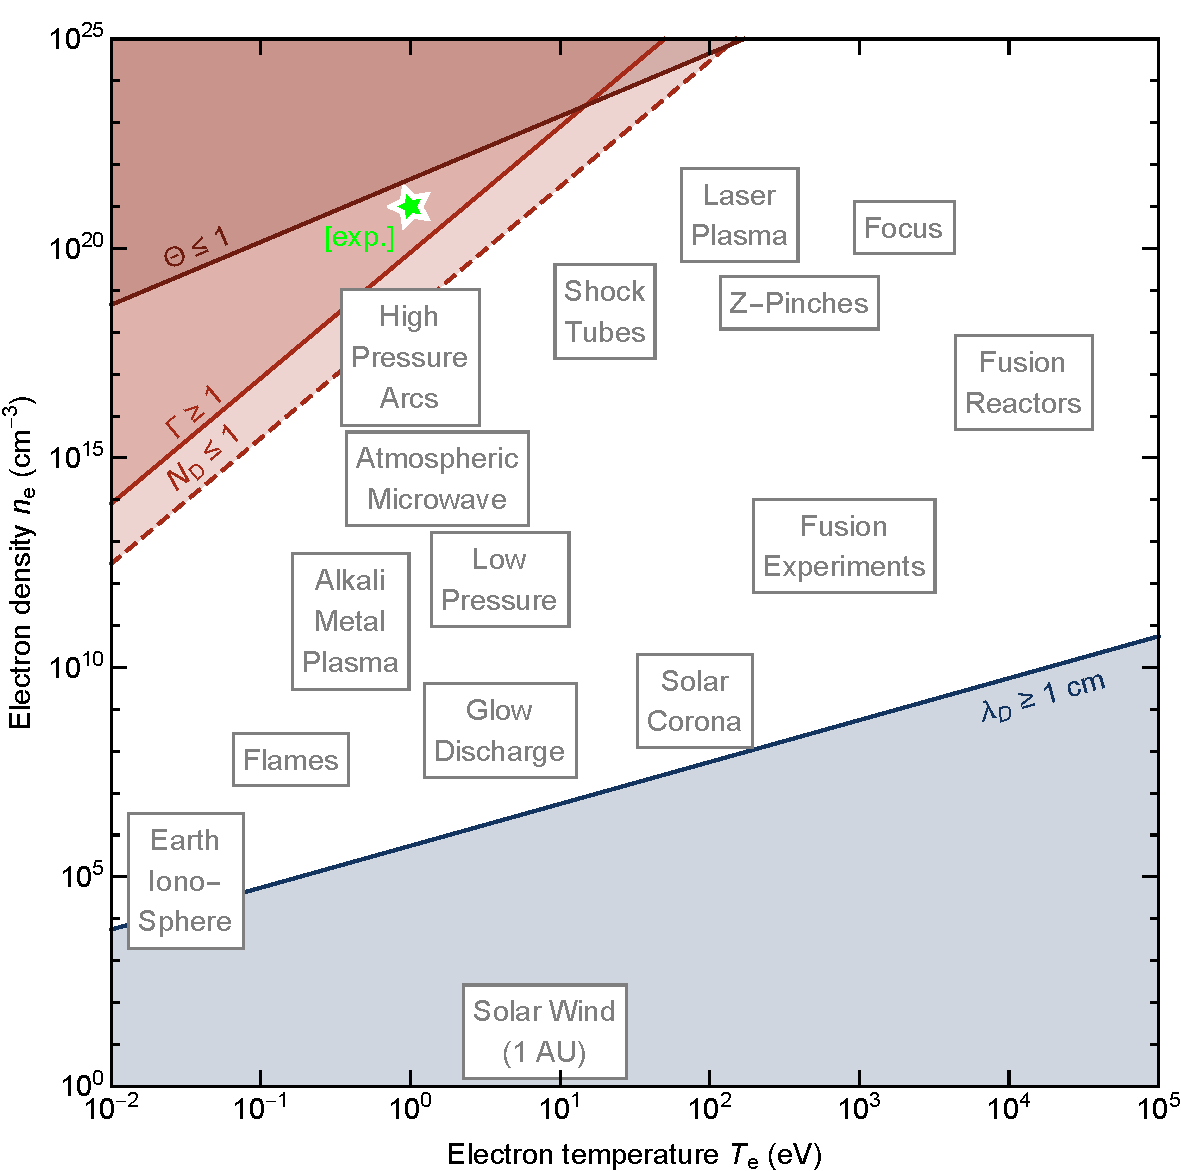
\includegraphics[width=100mm]{figures/ch1/taxonomy/taxonomy.pdf}
\caption{Plasma taxonomy retrieved from \cite{huba1998nrl}. The field of research in plasma physics is wide. The regime where the electron temperature or density is not extremely high or low has been traditionally studied. Strongly coupled plasmas are located in the top left corner of this phase diagram. Our experimental condition is shown with a green star.}
\label{fig:taxonomy}
\end{figure}

The various fields described above often have significantly different properties from the perspective of plasma physics \cite{huba1998nrl, bellan2008fundamentals}. So, it is helpful to systematically classify the types of plasmas, limiting the scope of the applicable theory and understanding it. The elements being discharged are diverse such as helium, argon, or xenon, and the types of particles composing the plasma are various including ions, neutral particles, and nanoparticles. However, the electron is at the center of it. In most cases, the electrons play the most important role in the generation and annihilation of plasma, so we can effectively classify plasma according to the conditions of electrons. Just as fluids are classified by drawing a phase diagram according to pressure, temperature, and density, plasma is generally classified according to the density and temperature of electrons. Qualitatively, the plasma used in semiconductor processing equipment has a slightly lower temperature and a slightly higher density than the solar corona. On the other hand, lightning has a slightly cooler temperature and much higher density (see Fig.\ref{fig:taxonomy}. More details will be discussed in Chap.\ref{sec:ch3-1}).

Traditionally, the regime where the electron temperature or density is not extremely high or low has been studied. However, recently, the growing versatility of experimental technologies such as lasers made it possible to explore deeper regimes. In particular, experimental research on low-temperature, high-density plasma has become a reality \cite{tsuda2000calculation, murillo2004strongly, harilal2004spatial, bataller2014blackbody, bataller2016observation, langin2019laser, kroker2020ultrafast}. It can indirectly address various scientific questions related to lightning phenomena in the thick atmosphere of Venus or the plasmas expected to exist at the cores of the planets \cite{ichimaru1982strongly, rogers2013strongly, kalman2013strongly, ichimaru2012strongly}.

The research topic of this thesis is the experimental study of low-temperature and high-density plasmas. In order to classify the regime more strictly, a plasma coupling parameter is introduced. The plasma coupling parameter is the ratio between the Coulomb potential energy and kinetic energy of the system. In the case of low-temperature and high-density, for instance, the average kinetic energy of electrons is small as the temperature is low, and there is a chance for the coupling parameter to increase. In addition, if the electron density is high, the average distance between the electrons becomes closer, and as a result, the potential energy of the system increases. By these two reinforcing influences, the high value of the coupling parameter is achieved. Technically, a plasma with a coupling parameter greater than unity is defined as a strongly coupled plasma -- further details will be given in Chap.\ref{sec:ch3}. The strongly coupled plasmas are found in many objects such as stars, galaxies, white dwarf stars, cores of Jovian planets, lightening in the thick planetary atmospheres, and inertial confinement fusion \cite{ichimaru1982strongly, murillo2004strongly, ichimaru2012strongly}.

Recently, experimental research on strongly coupled plasma has been actively conducted. One of the typical characteristics of strongly coupled plasma is that the orbitals of particles overlap, and thereby, the ionization potential of atoms decreases as if the orbitals of atoms close together in a metal, electrons move to the conduction band and freely move around \cite{griem1962high, ciricosta2012direct}. This phenomenon is called pressure ionization. In these high-density plasmas, many traditional plasma theories do not work well \cite{murillo2004strongly, huebner2014opacity}.

In this study, a nanosecond laser pulse is focused on the high-pressure argon fluid at room temperature to generate a strongly coupled plasma with low-temperature and high-density. The argon fluid is in a supercritical state under this condition. Strongly coupled plasma experiments under similar conditions have been performed by several groups and reported \cite{tsuda2000calculation, harilal2004spatial, bataller2014blackbody, bataller2016observation}. However, in this study, there is one major difference from the previous experiments. It is related to the inhomogeneity of the target medium. For instance, inhomogeneous supercritical argon fluid is adopted for the target medium, and the medium inhomogeneity creates several important differences.

The argon fluid undergoes an instantaneous compression-expansion process while filling the chamber, and the instantaneously adiabatic expanded fluid rapidly cools and liquefies \cite{lee2021quasi}. The supercritical fluid after the compression process contains a large amount of liquefied argon droplets with a size of several to hundreds of nanometers. A large number of argon droplets slowly evaporate over an hour in the supercritical medium. According to the textbook definition of supercritical fluid, it is a homogeneous medium without surface tension, but in actual experiments, it has been observed that at least, two different phases coexist for a long time.

These liquified particles play an important role on the particle kinetics of the plasma generated in the phase coexisting medium. Submicron-sized argon droplets in the plasma usually have a large number of electrons attached to them. Over time, these electrons emit light and disappear as they recombine with the surrounding ions. However, there is no robust theory on how these mesoscopic particles become charged and disappear in a strongly coupled plasma. Our experiment shows that mesoscopic particles in the strongly coupled plasma temporarily store the electrons on their surfaces.

In addition, argon droplets have a profound effect on the energy transport of the plasma, as well. The kinetic energy of electrons in plasma is mainly released through elastic collisions with large particles such as atoms or ions around them. When the high-temperature electrons are initially generated, energy is taken away from the electrons when they collide with the surrounding heavy particles, raising the temperature of the medium itself. However, this process slows down if the average mass ratio of the electrons to the surrounding fluid particles becomes large \cite{bellan2008fundamentals}. In the extreme, when an electron collides with an object of infinite mass, the electron may only change its direction of motion and does not lose energy. Thus, in a fluid containing large amounts of mesoscopic particles that are much larger and heavier than individual atoms, the electrons release less kinetic energy for each collision, resulting in slower electron-to-fluid energy transport. As a result, the argon droplets in the supercritical fluid slow down the energy released from the electrons and thereby enhance the energy confinement of the plasma.

Recalling that many strongly coupled plasmas in nature will occur in the inhomogeneous media, this finding provides an expanded perspective on the existing knowledge about such plasmas. In addition, when conducting an experimental exploration of dense plasmas, short pulse type experiments are mainly performed because it is difficult to maintain high energy density for a long time. As the medium inhomogeneity prolongs the plasma lifetime by delaying the energy release time, and as a result, our system can reduce the experimental difficulty and serve as a platform for applied research.

The experimental apparatus we implemented can be exploited for other practical applications as well. Plasma generated from high-pressure or supercritical fluid has close connections to various applications. One of the popular applications of plasma is material synthesis \cite{vollath2008plasma, kramer2015cold, stauss2015review}. Since the particle energy in the plasma is elevated, plasma is widely applied as an environment for synthesizing materials that are difficult to be formed under usual conditions. The strongly coupled plasma with enhanced charge and energy confinements by the medium inhomogeneity may improve energy efficiency and harvest rate in such applications. As mentioned, this study not only provides interesting observational results related to strongly coupled plasma in the inhomogeneous medium, but can also be used in various fields of application. \\

The thesis proceeds as follows:
\begin{itemize}
  \item Chap.\ref{sec:ch2} introduces the recent observation of quasi-equilibrium coexistence of liquid-like and gas-like phases in the supercritical fluid.
  \item Chap.\ref{sec:ch3} reviews the phenomena associated with the strongly coupled plasma and compares them with classical ideal plasmas.
  \item Chap.\ref{sec:ch4} presents the experimental results that show the role of mesoscopic particles in the strongly coupled plasmas.
  \item Chap.\ref{sec:ch5} concludes with a summary and outlook for the further implications of the medium inhomogeneity on the strongly coupled plasmas.
  \item Additionally, Appendix.\ref{sec:ap7} covers a side topic regarding an atmospheric pressure plasma.
\end{itemize}
